\documentclass[10pt]{beamer}
%\usepackage[slovene]{babel}
\usepackage[utf8]{inputenc}
\usepackage[T1]{fontenc}
\usepackage{lmodern}
\usepackage{mathptmx}
\usepackage{helvet}
\usepackage{courier}
\usepackage{hyperref}
\usepackage{wrapfig}
\usepackage{tikz}
\usepackage{tcolorbox}

\usetheme{CambridgeUS}

\begin{document}

\title[Kazalniki ekonomske neenakosti]{Kazalniki ekonomske neenakosti}
\author{Eva Deželak, Žan Jarc, Veronika Sovdat in Ines Šilc}
\institute [FMF]{ Fakulteta za matematiko in fiziko}

\begin{frame}
	\titlepage
\end {frame}

\begin{frame}
Vsebina predavanja:
	\begin{itemize}
		\item Definicije osnovnih pojmov
		\item Tekma med izobraževanjem in tehnologijo
		\item Posamezni kazalniki neenakosti
			\begin{itemize}
				\item Prag revščine
				\item Lorenzova krivulja
				\item Ginijev koeficient
				\item Palmovo razmerje
			\end{itemize}
		\item Ekonomska neenakost doma in po svetu
		\item Ekonomska neenakost in demokracija
	\end{itemize}
\end {frame}

\begin{frame}
\frametitle{Definicije osnovnih pojmov}
\begin{itemize}
\item \textbf{Državni dohodek} je vsota vseh dohodkov, ki so na voljo prebivalcem neke države v danem letu, ne glede na klasifikacijo dohodkov.
$$
\textbf{Državni dohodek} = \textbf{BDP} - \textbf{cena kapitala} + \textbf{neto dobiček iz tujine}
$$
\item \textbf{Državno premoženje} je vsota privatnega in javnega premoženja.
$$
\textbf{Državno premoženje}~=~\textit{domači kapital}~+~\textit{neto tuji kapital}
$$
\item Neenakost v odnosu do dela in kapitala. Plače so ena oblika dohodka iz dela, dohodek iz kapitala pa predstavlja vse prihodke, ki jih ima lahko nek posameznik od kapitala, to so lahko na primer najemnine, dividende, obresti\dots
\end{itemize}
\end{frame}

\begin{frame}
\frametitle{Tekma med izobraževanjem in tehnologijo}
\begin{itemize}
\item Teorija ima dve predpostavki:
\begin{enumerate}
\item Plača delavca je enaka njegovi \textbf{mejni produktivnosti}.
\item Produktivnost delavca je odvisna od njegovih spretnosti in strokovnega znanja ter \textbf{ponudbi} teh spretnosti v dani družbi.
\end{enumerate}


\item Teorija o tekmi med izobraževanjem temelji predvsem na ponudbi in povpraševanju strokovnega znanja v neki državi. 
\item Tehnološki napredek je odvisen od hitrosti inovacij in hitrosti implementacije teh inovacij. Ponavadi dvigne povpraševanje za nova strokovna znanja in ustvari nova delovna mesta.


\item Pomanjkljivosti:
\begin{enumerate}
\item Plača $\neq$ mejna produktivnost
\item Ne razloži gromozanskih razlik med plačami direktorjev in delavci podjetja.
\end{enumerate}
\end{itemize}
\end{frame}

\begin{frame}
\frametitle{Ginijev koeficient}

\begin{columns}[T]
    \begin{column}{.5\textwidth}
     \begin{block}{}
\begin{itemize}
\item Italijanski statistik Corrado Gini (1884 - 1965).
\item Število 0 predstavlja popolno enakost, število 1 pa popolno neenakost. 
\item PRIMER: 10 \% svetovnega prebivalstva si lasti 87,7 \% celotnega svetovnega bogastva.
\end{itemize}
    \end{block}{}
    \end{column}
    \begin{column}{.5\textwidth}
    \begin{block}{Corrado Gini}
    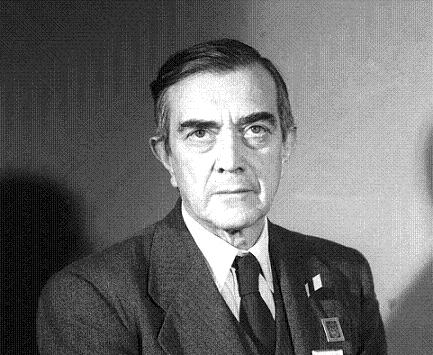
\includegraphics[width=0.9\textwidth]{./slike/corrado-gini.jpg}
    \end{block}{}
    \end{column}
  \end{columns}
\end{frame}

\begin{frame}
\frametitle{Lorenzova krivulja}
\begin{itemize}
\item Populacija velikosti N, količina Q. 
\item Z L(p) označimo del količine Q, ki si jo lasti del populacije v prvem p-tem deležu.
\item Graf funkcije L(p) imenujemo \textbf{Lorenzova krivulja}.
\item Popolna enakomerna porazdelitev premoženja: L(p) = p.
$$\Rightarrow 0 \leq L(p) \leq p$$
\begin{tcolorbox}[colback=black!5,colframe=red!40!black,title=Ginijev koeficient]
$$G := 2 \cdot \int_{0}^{1} (p - L(P)) dp$$
\end{tcolorbox}
\item Ker je  $0 \leq \int_{0}^{1} (p - L(P)) dp \leq \int_{0}^{1} p dp = \frac{1}{2}$, je $G \in [0, 1].$
\end{itemize}
\end{frame}

\begin{frame}
\frametitle{Ekonomska neenakost doma in po svetu}
\begin{figure}
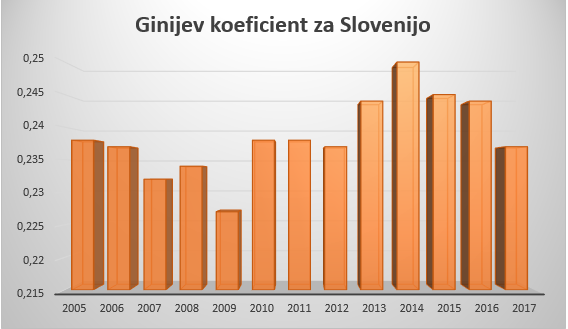
\includegraphics[width= \linewidth]{./slike/gini-slo.PNG}
\end{figure}
\end{frame}

\begin{frame}
\frametitle{Ekonomska neenakost doma in po svetu}
\begin{figure}
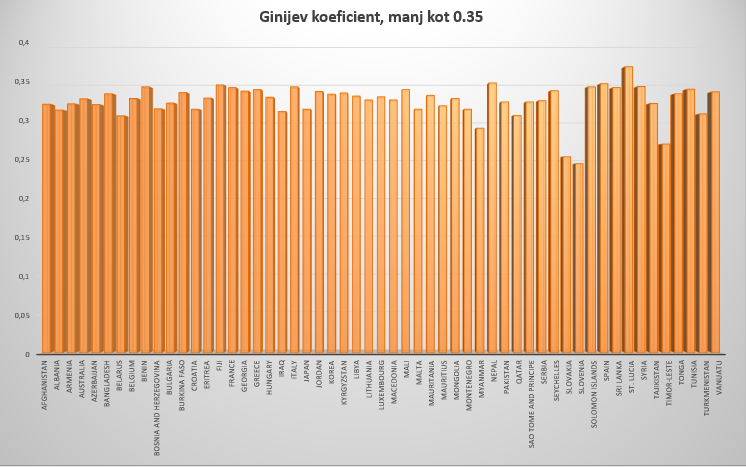
\includegraphics[height=.3 \textwidth, width = .7\linewidth]{./slike/gini-manj-07.PNG}
\hspace{0.3\textwidth}
\hfill
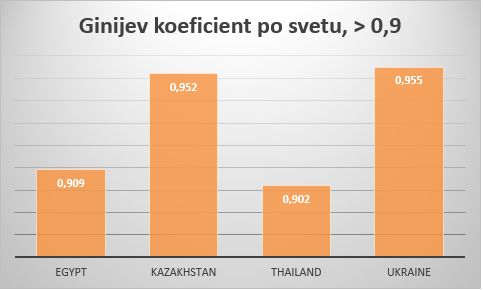
\includegraphics[height=.3 \textwidth, width = .6\linewidth]{./slike/gini-vec-09.PNG}
\end{figure}
\end{frame}





\begin{frame}
\frametitle{Palmovo razmerje}
\begin{itemize}
\item Kazalnik ekonomske neenakosti:

\begin{itemize}
\item $b := \textrm{delež dohodka, ki pripada 10\% prebivalstva z najvišjim dohodkom},$
\item $r := \textrm{delež dohodka, ki pripada 40\% prebivalstva z najnižjim dohodkom},$
\end{itemize}
$$
\textrm{Palmovo razmerje} := \frac{b}{r}.
$$

\item Lastnosti:
\begin{itemize}
\item osredotoči se na krajišča (na najrevnejše in najbogatejše prebivalstvo),
\item odzivno na visoko neenakost (Ginijev koeficijent opazi samo nizko neenakost),
\item preprost izračun.
\end{itemize}
\end{itemize}
\end{frame}

\begin{frame}
\frametitle{Graf: Palmovo razmerje in Ginijev koeficijent}
\begin{figure}
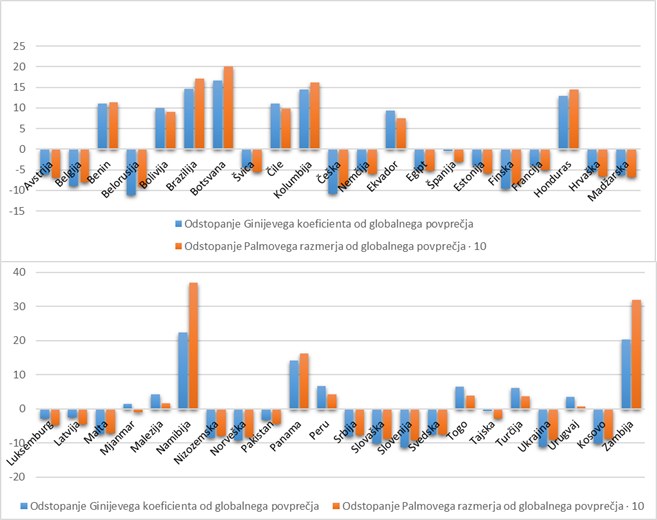
\includegraphics[scale = 0.87]{./slike/gini_palma.png}
\end{figure}

\end{frame}



\begin{frame}
\frametitle{Indikatorji revščine in posledično kazatelji neenakosti}
\begin{itemize}
\item \textbf{Stopnja tveganja revščine} - procent ljudi, ki živijo pod pragom revščine.

\item \textbf{Poverty gap index (PGI)}:
\begin{itemize}
\item $N := \textrm{število prebivalcev}$ ,
\item $q := \textrm{število prebivalcev, ki živijo pod pragom revščine}$,
\item $z := \textrm{prag revščine}$,
\item $q_i := \textrm{dohodek revnega prebivalca i}$,
\end{itemize}
$$
PGI = 1/N \sum_{j=1}^q (\frac{z-y_i}{z}).
$$
\end{itemize}
\end{frame}


\begin{frame}
\frametitle{Graf: Stopnja tveganja revščine in Ginijev koeficijent}
\begin{figure}
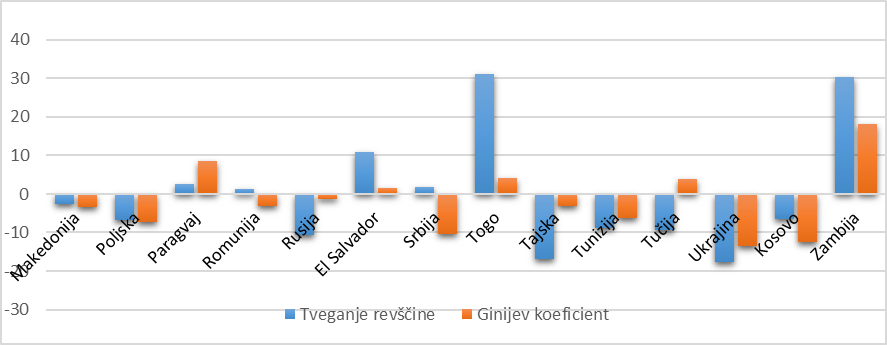
\includegraphics[scale = 0.8]{./slike/gini_revscina.png}
\end{figure}

\end{frame}









\begin{frame}
\frametitle{Viri}
	\begin{itemize}
		\item
			\label{Pickety}
			T.~Pickety, \emph{Capital in the twenty-first century}, The Belknap Press of 						Harvard University Press, London, 2014.

		\item 
			\label{Razdelitev premoženja}
			\emph{Distribution of wealth}, v: Wikipedia, The Free Encyclopedia, [ogled 							20.~4.~2019], dostopno na \url{https://en.wikipedia.org/w/index.php?								title=Distribution_of_wealth&oldid=854198883}.

		\item 
			\label{Metrike ekonomske neenakosti}
			\emph{Income inequality metrics}, v: Wikipedia, The Free Encyclopedia, [ogled 					20.~4.~2019], dostopno na \url{https://en.wikipedia.org/w/index.php?								title=Income_inequality_metrics&oldid=853906711}.

\item
\emph{Ginijev koeficient}, Janja Trogar, [ogled 3.~5.~2019], dostopno na \url{https://repozitorij.uni-lj.si/IzpisGradiva.php?id=97164}.

\item
\emph{Statistični urad RS}, Neenakost porazdelitve dohodka - Ginijev količnik (\%), Slovenija, letno, [ogled 4.~5.~2019], dostopno na \url{https://pxweb.stat.si/pxweb/Dialog/varval.asp?ma=0867312S&ti=&path=../Database/Dem_soc/08_zivljenjska_raven/08_silc_kazalniki_revsc/15_08673_porazdel_dohodka/&lang=2}.
\end{itemize}
\end {frame}










\end{document}